% pdflatex --shell-escape TalkIcnc
\documentclass[10pt]{beamer}
\usepackage[english]{babel} 
\usepackage[timeinterval=10]{tdclock}
\setbeamertemplate{navigation symbols}{} %no nav symbols
\usepackage{tikz}
\usetikzlibrary{patterns,decorations,fadings,shapes,backgrounds,mindmap} 
\usepackage{animate}
\usepackage{color}
\usepackage{multimedia}
\usepackage{beamerthemesplit}
%\usefonttheme{professionalfonts}

% Color "correction"
% See http://tug.org/pipermail/pdftex/2007-December/007457.html
\pdfpageattr {/Group << /S /Transparency /I true /CS /DeviceRGB>>}

% Choose font
% -----------
%\usepackage{fontspec} 
%\setsansfont{GillSans}

% Add frame number/frame total on footline (right)
% ------------------------------------------------
\definecolor{myblue}{rgb}{0,0.2,0.4}
\newcommand*\oldinsertshorttitle{}%
\let\oldinsertshorttitle\insertshorttitle%
\renewcommand*\insertshorttitle{%
  \oldinsertshorttitle\hfill%
  \insertframenumber}



% Commands
% --------
\newcommand{\reflection}[2][\textwidth]
{
  \begin{tikzpicture}[inner sep=0.1mm]
    \pgfdeclareimage[width=#1]{pic}{#2}
    \node [draw=black,line width=.1mm,anchor=south west, yscale= 1]
           (image) at (0,0) {\pgfuseimage{pic}};
    \clip [scope fading=south] (0,0) rectangle (1.01*#1,-7.5mm);
    \node [draw=black,line width=.1mm,anchor=south west,yscale=-1,opacity=.25]
           (image) at (0,-.1mm) {\pgfuseimage{pic}};
  \end{tikzpicture}
}

\newcommand{\image}[2][\textwidth]
{
  \begin{tikzpicture}[inner sep=0.1mm]
    \pgfdeclareimage[width=#1]{pic}{#2}
    \node [draw=black,line width=.1mm,anchor=south west, yscale= 1]
           (image) at (0,0) {\pgfuseimage{pic}};
  \end{tikzpicture}
}




% Docmument title, author, date and institution
% ---------------------------------------------
\title[Dynamiques et D\'ecisions]{Mod\'elisation de Populations Neuronales pour l'Int\'egration Visuo-motrice:\\Dynamiques et D\'ecisions}
\date[soutenance]{ Th\`ese pr\'esent\'ee le 26 septembre 2012}
\author{\em Wahiba TAOUALI}


\tikzstyle{mybox} = [draw=black, opacity=1, fill opacity=.5, thick, rectangle, inner sep=5pt]  


% =============================================================================
\begin{document}

% For every picture that defines or uses external nodes, you'll have to
% apply the 'remember picture' style. To avoid some typing, we'll apply
% the style to all pictures.
%\tikzstyle{every picture}+=[remember picture]

% By default all math in TikZ nodes are set in inline mode. Change this to
% displaystyle so that we don't get small fractions.
%\everymath{\displaystyle}


% =============================================================================
\begin{frame}
  \titlepage
  \initclock


\includegraphics [width=2cm]{lorraine-universite}
\hspace*{0.2\textwidth}

\includegraphics [width=2cm]{loria}
\hspace*{0.05\textwidth}
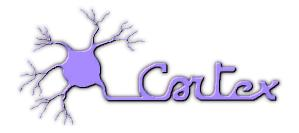
\includegraphics [width=2cm]{cortex}
\hspace*{0.05\textwidth}

\includegraphics [width=2cm]{inria}\\

\end{frame}


\section{Contexte g\'en\'eral}
\begin{frame}
  \frametitle{Les sciences cognitives:}
$\to$ Description, explication et simulation des m\'ecanismes mentaux.
	 \begin{tikzpicture}
	      \pgfdeclareimage[width=1.\textwidth,interpolate=true]{pic}{figures/cognition}
	      \node [] (image) at (0,0) {\pgfuseimage{pic}};
	    \end{tikzpicture}
\end{frame}
%\end{section}


\begin{frame}
  \frametitle{L'\'enaction: l'action dans la perception}
\begin{columns}
    \begin{column}{0.5\textwidth}
  \begin{block}{}
\hspace*{0.2\textwidth}
\vspace{0.3cm}
    \begin{tikzpicture}
      \pgfdeclareimage[width=0.4\textwidth,interpolate=true]{pic}{figures/action}
      \node [] (image) at (0,0)  {\pgfuseimage{pic}};
    \end{tikzpicture}
    \begin{tikzpicture}
      \pgfdeclareimage[width=0.4\textwidth,interpolate=true]{pic}{figures/oeil\string_cerveau}
      \node [] (image) at (0,0)  {\pgfuseimage{pic}};
    \end{tikzpicture}

    \``During visual search, the brain performs a sophisticated deployment of {\color {blue} {eye movements}} (saccadic actions) to gather information to subserve perceptual judgments.''\begin{flushright}
      {\footnotesize  Eckstein et al., J. Neuroscience, 2007 }
    \end{flushright}
  \end{block}
\end{column}
\begin{column}{0.5\textwidth}
 \begin{block}{}
``{\color {blue} {Perception}} is not something that happens to us, or in us, it is something {\color {blue} {we do}}.''
    \begin{flushright}
      {\footnotesize A. No\"e, Action in Perception, 2006}
    \end{flushright}
\vspace{0.5cm}
\hspace*{0.2\textwidth}
    \begin{tikzpicture}
      \pgfdeclareimage[width=0.7\textwidth,interpolate=true]{pic}{figures/Maldonaldo}
      \node [] (image) at (0,0) {\pgfuseimage{pic}};
    \end{tikzpicture}
  \end{block}
\end{column}
\end{columns}

\end{frame}
%%%%%%%%%%%%%%%%%%%%%%%%%%%%%%%%%%%%%%%%%%%%%%%%%%%%%%%%%%%%%%%%%%%%%%%%%%%
\begin{frame}
  \frametitle{Probl\'ematique}

``La {\color{blue}perception} et l'{\color{blue}action}, le perceptif et le moteur sont li\'es en tant que motifs {\color{red}\'emergents} qui se {\color{blue}s\'electionnent} mutuellement.'' [Varela, 1993]\\
 \vspace{1cm} \hspace{4cm}Syst\`eme {\color {myblue}\'enactif} \\
\begin{columns}
    \begin{column}{0.85\textwidth}
\begin {itemize}
\item[$\bullet$] Syst\`eme {\color {myblue}dynamique incarn\'e}:\\
 interaction {\color {blue}locale} entre unit\'es {\color {blue}\'el\'ementaires homog\`enes}:\\
$\to$ syst\`eme r\'eactif / d\'ecision ``structurelle''
\item[$\bullet$] Syst\`eme {\color {myblue}dynamique situ\'e}:\\
interaction {\color {blue}globale}  entre flux {\color {blue} h\'et\'erog\`enes}:\\
$\to$ syst\`eme actif / d\'ecision ``modul\'ee''
\end {itemize}  
\end{column}
    \begin{column}{0.4\textwidth}

    \begin{tikzpicture}
      \pgfdeclareimage[width=0.8\textwidth,interpolate=true]{pic}{figures/complexe}
      \node [] (image) at (0,0)  {\pgfuseimage{pic}};
    \end{tikzpicture}
\end{column}
\end{columns}

 \vspace{0.5cm}
{\color {blue} Probl\'ematique:}\\
Comment passer de {\color {red}``l'\'emergence r\'eactive''} \`a {\color {red}``l'\'emergence active''}?\\

\end{frame}
%%%%%%%%%%%%%%%%%%%%%%%%%%%%%%%%%%%%%%%%%%%%%%%%%%%%%%%%%%%%


%\textit  {``l'intelligence artificielle [...] concerne la recherche des moyens susceptibles de doter les syst\`emes informatiques de capacit\'es intellectuelles comparables \`a celles des \^etres humains[Simon,1979]''}
\begin{frame}
  \frametitle{Objectifs}
\begin{itemize}
\item<1->  {\color {blue}Objectif 1}: {\color {myblue}comment des comportements complexes \'emergent d'un calcul local et homog\`ene ?}
\begin{itemize}
\item<2-> calculatoire: hypoth\`eses sur l'organisation spatiale et temporelle\\
$\to$ La CNFT
\item<3->  fonctionnel: s\'election structurelle de cibles visuelles\\
$\to$ Le colliculus sup\'erieur
\end{itemize}
\item<4-> {\color {blue}Objectif 2}: {\color {myblue}comment une s\'election active (motiv\'ee) peut \'emerger de l'interaction entre plusieurs boucles et flux h\'et\'erog\`enes?} \\
%\begin{itemize}
%\item<2> L'interaction entre des boucles diff\'erentes et des flux h\'et\'erog\`enes implicant le contexte sensoriel, \'emotif et temporel\\
$\to$  Les ganglions de la base
\end{itemize}
\end{frame}


%%%%%%%%%%%%%%%%%%%%%%%%%%%%%%
\begin{frame}
  \frametitle{Approches}
\begin{itemize}

\item[$\bullet$] donn\'ees biologiques + exp\'eriences comportementales \\{\em {\color {blue} $\to$}} hypoth\`eses + param\`etres 
\item[$\bullet$] mod\`eles + simulations \\{\em {\color {blue} $\to$}} comparaisons + pr\'edictions

\end{itemize}
\begin{center}
\begin{tikzpicture}
      \pgfdeclareimage[width=0.4\textwidth,interpolate=true]{pic}{figures/chercheur}
      \node [] (image) at (0,0) {\pgfuseimage{pic}};
    \end{tikzpicture}

\end{center}

\end{frame}


%%%%%%%%%%%%
\begin{frame}
  \frametitle{Section 1}
\begin{center}
{{\color{blue}\'Emergence R\'eactive:}\\
Encodage de saccades oculaires }
\end{center}
\end{frame}
\begin{frame}
  \frametitle{Le syst\`eme visuo-moteur: s\'election de cibles visuelles}
\begin{itemize}
\item Organisation complexe. 
\begin{tikzpicture}<5->
      \pgfdeclareimage[width=0.8\textwidth,interpolate=true]{pic}{figures/Structures2}
      \node [] (image) at (0,0) {\pgfuseimage{pic}};
    \end{tikzpicture}
\end{itemize}
\end{frame}
\begin{frame}
  \frametitle{Le colliculus sup\'erieur}
\begin{columns}
\begin{column}{0.7\textwidth}
\begin{itemize}
\item Petite structure sous-corticale laminaire multimodale
\item Des mod\`eles complexes\\ (typologie, topographie, dynamique)
\item Hypoth\`eses communes:
\begin{itemize}
\item[$\bullet$] {\color{blue} Projection r\'etinienne logarithmique}\\
\small{[Optican 1995, Lef\`evre 1998, Trappenberg 2001, Nakahara 2006, Marino 2008...]}
\item[$\bullet$] {\color{blue}Carte homog\`ene computationnelle : connectivit\'e lat\'erale}\\
\small{[Droulez et Berthoz 1991, Arai et al 1994, Gancarz et Grossberg 1999, Trappenberg 2001, Schneider and Erlhager 2002, Nakahara et al 2006, Marino 2012...]}
\end{itemize}
\end{itemize}
\end{column}
\begin{column}{0.4\textwidth}
\begin{tikzpicture}
      \pgfdeclareimage[width=1\textwidth,interpolate=true]{pic}{figures/col}
      \node [] (image) at (0,0) {\pgfuseimage{pic}};
\end{tikzpicture}
\begin{flushright}{\footnotesize [lecerveau.mcgill.ca]}\end{flushright}
\end{column}
\end{columns}
\vspace{0.5cm}
$\to$ Un mod\`ele ``unificateur'':\\ {\color{purple} comportements \'emergents de ces hypoth\`eses ``structurelles'' ?}
\end{frame}

%***********************************************************************************************************
\begin{frame}
  \frametitle{Mod\`ele minimaliste: hypoth\`eses et m\'ethodes}
\begin{itemize}
\item[$\bullet$] Codage topographique [Schiller et al 1972, Wurtz et Goldberg 1972] \\
$\to$ projection logarithmique [Ottes et al 1986]
\end{itemize}
%\item[$\bullet$] Connectivit\'e lat\'erale : diff\'erence de gaussiennes 
%\begin{tikzpicture}
%      \pgfdeclareimage[width=0.25\textwidth,interpolate=true]{pic}{figures/gauss}
%      \node [] (image) at (0,0) {\pgfuseimage{pic}};
%    \end{tikzpicture}
%\item[$\bullet$] Les influences des aires corticales, des ganglions de la base et du cervelet ne sont pas consid\'er\'ees 
%\item<6->[$\bullet$] Un seul colliculus est consid\'er\'e
%\end{itemize}
\begin{center}
\begin{tikzpicture}
      \pgfdeclareimage[width=0.7\textwidth,interpolate=true]{pic}{figures/single-stimulus-1}
      \node [] (image) at (0,0) {\pgfuseimage{pic}};
    \end{tikzpicture}
\end{center}
\end{frame}
\begin{frame}
  \frametitle{Mod\`ele minimaliste: hypoth\`eses et m\'ethodes}
\begin{itemize}
\item[$\bullet$] Codage par population \\
$\to$ champ de neurones dynamique: connectivit\'e lat\'erale  (CNFT)
\end{itemize}
%\item[$\bullet$] Connectivit\'e lat\'erale : diff\'erence de gaussiennes 
%\begin{tikzpicture}
%      \pgfdeclareimage[width=0.25\textwidth,interpolate=true]{pic}{figures/gauss}
%      \node [] (image) at (0,0) {\pgfuseimage{pic}};
%    \end{tikzpicture}
%\item[$\bullet$] Les influences des aires corticales, des ganglions de la base et du cervelet ne sont pas consid\'er\'ees 
%\item<6->[$\bullet$] Un seul colliculus est consid\'er\'e
%\end{itemize}
\begin{center}
\begin{tikzpicture}
      \pgfdeclareimage[width=0.5\textwidth,interpolate=true]{pic}{figures/DoG}
      \node [] (image) at (0,0) {\pgfuseimage{pic}};
    \end{tikzpicture}\begin{tikzpicture}
      \pgfdeclareimage[width=0.5\textwidth,interpolate=true]{pic}{figures/weights-profile-1}
      \node [] (image) at (0,0) {\pgfuseimage{pic}};
    \end{tikzpicture}
\end{center}
\end{frame}
%**********************************************************************************************************
\begin{frame}
  \frametitle{Th\'eorie des champs de neurones continus (CNFT)}

\begin{itemize}
\item Cortex humain: $10^5$ neurones/$mm^3$ [C.Koch 2004]\\
{\color {blue}$\to$} une couche de neurones est {\color{blue}un continuum} dans l'espace [Wilson and Cowan 1973].
\item<1-> Suivant les notations introduites par [Amari, 1977], l'\'evolution du {\color{blue} potentiel de membrane} $u(x,t)$ à la position $x$ est donn\'ee par:
    \vspace{-3mm}
    %\everymath{\displaystyle}
    \begin{small}
      \begin{equation*}
        \tikz[baseline]{
          \path[use as bounding box] (0,0) rectangle (.2,1);
          \node[fill=blue!10,anchor=base,
            rounded corners,pin={[blue,scale=.75]below:constante de temps}]
               {$\tau$};
        }
        \cdot \frac{\partial{u(x,t)}}{\partial{t}} = 
        \tikz[baseline]{
          \node[fill=blue!10,anchor=base,
            rounded corners,pin={[blue,scale=.75]below:terme de fuite}]
               {$-u(x,t)$};
        } + \int_{-\infty}^{+\infty}
        \tikz[baseline]{
          \node[fill=blue!10,anchor=base,
            rounded corners,pin={[blue,scale=.75]below:interaction lat\'erale}] (t1)
               {$w(x-y) \cdot f(u(y,t))$};
        } dy +
        \tikz[baseline]{
          \node[fill=blue!10,anchor=base,
            rounded corners,pin={[blue,scale=.75]below:entr\'ee}]
               {$I(x)$};
        } + 
        \tikz[baseline]{
          \path[use as bounding box] (-.25,0) rectangle (0,1);
          \node[fill=blue!10,anchor=base,
            rounded corners,pin={[blue,scale=.75]below:seuil}]
               {$h$};
        }
      \end{equation*}
    \end{small}
\begin{itemize}
\item[$\bullet$]<2-> int\'egration num\'erique: {\em {\color {myblue}du continu au discret}}
\item[$\bullet$]<3-> calcul distribu\'e: {\em {\color {myblue} a-t-on besoin d'une horloge centrale?}}
[Taouali et al 2011]%qui est à votre disposition dans le manuscrit
\end{itemize}
\item<4-> profils de connexions : {\color{blue}paradigme de comp\'etition} robuste et rapide
\end{itemize}

\end{frame}
\begin{frame}
  \frametitle{Mod\`ele minimaliste: r\'esultats}
\begin{itemize}
\item S\'election d'{\color {blue}une} sous-population {\color {blue}st\'er\'eotyp\'ee}: \'etendue spatiale
\end{itemize}
\begin{center}
\begin{tikzpicture}
      \pgfdeclareimage[width=1.\textwidth,interpolate=true]{pic}{figures/colliculus-1}
      \node [] (image) at (0,0) {\pgfuseimage{pic}};
    \end{tikzpicture}
\end{center}
\begin{itemize}
\item[$\bullet$]Num\'erique: activation r\'esultante stable [Amari,1977]
\item[$\bullet$]Biologique: activation st\'er\'eotyp\'ee [Anderson, 1998]
\end{itemize}

\end{frame}
\begin{frame}
  \frametitle{Mod\`ele minimaliste: r\'esultats}
\begin{itemize}
\item {\color{myblue}Exactitude du codage par population}
\end{itemize}

\hspace{2cm}\begin{tikzpicture}
      \pgfdeclareimage[width=0.6\textwidth,interpolate=true]{pic}{figures/lesion-1}
      \node [] (image) at (0,0) {\pgfuseimage{pic}};
    \end{tikzpicture}
\end{frame}
\begin{frame}
  \frametitle{Mod\`ele minimaliste: r\'esultats}
\begin{itemize}
\item d\'ecroissance du rostral vers le caudal [Munoz and Wurtz 1995].
\\{\color {blue} $\to$} effet de la projection logarithmique et l'inhibition globale
\item un maximum d'activation pour une direction pr\'ef\'erentielle 
\end{itemize}
\begin{columns}
    \begin{column}{0.8\textwidth}
\begin{center}
\begin{tikzpicture}
      \pgfdeclareimage[width=1.\textwidth,interpolate=true]{pic}{figures/SC\string_accord1}
      \node [] (image) at (0,0) {\pgfuseimage{pic}};
    \end{tikzpicture}
\end{center}
\end{column}
\begin{column}{0.4\textwidth}
\begin{center}
\begin{tikzpicture}
      \pgfdeclareimage[width=0.7\textwidth,interpolate=true]{pic}{figures/accord}
      \node [] (image) at (0,0) {\pgfuseimage{pic}};
    \end{tikzpicture}
\end{center}
\end{column}
\end{columns}
\end{frame}
\begin{frame}
  \frametitle{Mod\`ele minimaliste: r\'esultats}
\begin{columns}
\begin{column}{0.5\textwidth}
\begin{itemize}
\item la projection logarithmique: s\'election fov\'eale [Findlay and Walker 1999]
\item $< 50^\circ$: Effet global [Coren and Hoenig 1972]
\begin{tikzpicture}
      \pgfdeclareimage[width=0.5\textwidth,interpolate=true]{pic}{figures/distractor-effect-3}
      \node [] (image) at (0,0) {\pgfuseimage{pic}};
    \end{tikzpicture}
\item $> 50^\circ$: Effet distracteur distant [Levy-schoen 1969]

\begin{tikzpicture}
      \pgfdeclareimage[width=0.5\textwidth,interpolate=true]{pic}{figures/distractor-effect-2}
      \node [] (image) at (0,0) {\pgfuseimage{pic}};
    \end{tikzpicture}
\end{itemize}
\end{column}
\begin{column}{0.6\textwidth}
\begin{tikzpicture}
      \pgfdeclareimage[width=1.\textwidth,interpolate=true]{pic}{figures/stimulus-2}
      \node [] (image) at (0,0) {\pgfuseimage{pic}};
    \end{tikzpicture}
\begin{tikzpicture}
      \pgfdeclareimage[width=1.\textwidth,interpolate=true]{pic}{figures/stimulus-3}
      \node [] (image) at (0,0) {\pgfuseimage{pic}};
    \end{tikzpicture}
\begin{tikzpicture}
      \pgfdeclareimage[width=1.\textwidth,interpolate=true]{pic}{figures/stimulus-4}
      \node [] (image) at (0,0) {\pgfuseimage{pic}};
    \end{tikzpicture}
\end{column}
\end{columns}
\end{frame}
\begin{frame}
  \frametitle{Mod\`ele minimaliste: r\'esultats}
\begin{columns}
    \begin{column}{0.6\textwidth}
\begin{itemize}
\item Inactivation locale {\color {blue} $\to$} saccades \emph{Hypo-m\'etriques} et \emph{hyper-m\'etriques} comme report\'e dans
[Lee, Rohrer and Sparks 1988].
\end{itemize}
\begin{center}
\begin{tikzpicture}
      \pgfdeclareimage[width=0.8\textwidth,interpolate=true]{pic}{figures/lesion-3}
      \node [] (image) at (0,0) {\pgfuseimage{pic}};
    \end{tikzpicture}
\end{center}

\end{column}
    \begin{column}{0.4\textwidth}
\begin{tikzpicture}
      \pgfdeclareimage[width=\textwidth,interpolate=true]{pic}{figures/lee}
      \node [] (image) at (0,0) {\pgfuseimage{pic}};
    \end{tikzpicture}
\end{column}
\end{columns}
\end{frame}
\begin{frame}
  \frametitle{Mod\`ele minimaliste: pr\'edictions}
\begin{itemize}
\item Temps de r\'eponse (taille, excentricit\'e, intensit\'e)
\end{itemize}
\begin{columns}
\begin{column}{0.4\textwidth}
\begin{tikzpicture}
      \pgfdeclareimage[width=1\textwidth,interpolate=true]{pic}{figures/RT-size-B}
      \node [] (image) at (0,0) {\pgfuseimage{pic}};
    \end{tikzpicture}
\end{column}
\begin{column}{0.4\textwidth}
\begin{tikzpicture}
      \pgfdeclareimage[width=1\textwidth,interpolate=true]{pic}{figures/RT-magnitude-B}
      \node [] (image) at (0,0) {\pgfuseimage{pic}};
    \end{tikzpicture}
\end{column}
\begin{column}{0.4\textwidth}
\begin{tikzpicture}
      \pgfdeclareimage[width=1\textwidth,interpolate=true]{pic}{figures/RT-eccentricity-B}
      \node [] (image) at (0,0) {\pgfuseimage{pic}};
    \end{tikzpicture}
\end{column}
\end{columns}
\end{frame}
\begin{frame}
  \frametitle{Synth\`ese}
\begin{itemize}
\item<1-> un fonctionnement local et homog\`ene avec connectivit\'e lat\'erale
\item<2-> un flux s\'equentiel avec une topographie particuli\`ere: codage spatial
\item<3-> un mod\`ele de base simple et solide pour l'encodage de cibles visuelles\\
\begin{tikzpicture}
      \pgfdeclareimage[width=0.8\textwidth,interpolate=true]{pic}{figures/stimulus-2}
      \node [] (image) at (0,0) {\pgfuseimage{pic}};
    \end{tikzpicture}
\end{itemize}
\end{frame}
\begin{frame}
  \frametitle{Synth\`ese}
\begin{itemize} %transition
\item[$\bullet$]<1-> une {\color{blue}s\'election structurelle} impos\'ee par l'architecture intrins\`eque 
\item[$\bullet$]<2-> un syst\`eme dynamique {\color{blue}incarn\'e} [Varela]: r\'etine fov\'eale
\item[$\bullet$]<3-> un syst\`eme dynamique {\color{blue}situ\'e}: \\
\vspace{0.2cm}\hspace{0.2cm}{\color{red}Interaction active avec l'environnement et \'emergence active?}\\
\hspace{2cm}\begin{tikzpicture}
      \pgfdeclareimage[width=0.4\textwidth,interpolate=true]{pic}{figures/varela}
      \node [] (image) at (0,0) {\pgfuseimage{pic}};
    \end{tikzpicture}
\end{itemize}
\end{frame}
\begin{frame}
  \frametitle{Section 2}
\begin{center}
{{\color{blue}\'Emergence Active:}\\
S\'election de l'action}
\end{center}
\end{frame}
\begin{frame}{Section 2:}
\begin{center}
\begin{tikzpicture}
      \pgfdeclareimage[width=0.6\textwidth,interpolate=true]{pic}{figures/door}
      \node [] (image) at (0,0) {\pgfuseimage{pic}};
    \end{tikzpicture}
\end{center}

%\begin{itemize}
%\item explorer d'autres actions possibles
%\item consid\'erer le contexte: motivation, exp\'erience (flux)
%\item choisir une cible visuelle moins focale (une action moins fr\'equente) ?
%\end{itemize}
%$\to$ {\color{blue}Les ganglions de la base} 
\end{frame}
\begin{frame}
  \frametitle{S\'election active}
\begin{columns}
    \begin{column}{0.5\textwidth}

\hspace*{0.4\textwidth}
%\vspace{0.7cm}
    \begin{tikzpicture}
      \pgfdeclareimage[width=0.4\textwidth,interpolate=true]{pic}{figures/fruits}
      \node [] (image) at (0,0)  {\pgfuseimage{pic}};
    \end{tikzpicture}
\end{column}
    \begin{column}{0.5\textwidth}
\hspace*{0.3\textwidth}
    \begin{tikzpicture}
      \pgfdeclareimage[width=0.4\textwidth,interpolate=true]{pic}{figures/ane}
      \node [] (image) at (0,0)  {\pgfuseimage{pic}};
    \end{tikzpicture}
\end{column}
\end{columns}

 La {\color {blue} saillance}: 
\begin {itemize}
\item[$\bullet$] une monnaie commune
\item[$\bullet$] une valeur d'utilit\'e attribu\'ee ponctuellement
\item[$\bullet$] contexte sensoriel, \'emotif et temporel
\end {itemize}
 \hspace{2cm}\vspace{2cm}$\to$ les ganglions de la base
\end{frame}

\begin{frame}
  \frametitle{Les ganglions de la base (BG)}
Un ensemble de noyaux sous-corticaux : \\entr\'ees {\color{myblue}corticales} -- sorties {\color{myblue}thalamiques}
\begin{columns}
\begin{column}{0.5\textwidth}

\begin{itemize}
\item une structure d'entr\'ee: striatum ({\color{myblue}Str}:putamen+noyau caud\'e)
\item deux structures de sorties: pallidum interne ({\color{myblue}GPi}) et substance noire r\'eticul\'ee ({\color{myblue}SNr})
\item deux structures interm\'ediaires: noyau sous-thalamique ({\color{myblue}STN}) et pallidum externe ({\color{myblue}GPe})
\end{itemize}
\end{column}
\begin{column}{0.6\textwidth}
\begin{tikzpicture}
      \pgfdeclareimage[width=0.9\textwidth,interpolate=true]{pic}{figures/BG1}
      \node [] (image) at (0,0) {\pgfuseimage{pic}};
    \end{tikzpicture}
\end{column}
\end{columns}
\end{frame}

\begin{frame}
  \frametitle{Les BG: Organisation en circuits}

\begin{itemize}
\item plusieurs circuits/fonctions
\item r\^ole g\'en\'erique de s\'election de l'action
\end{itemize}
\begin{tikzpicture}
      \pgfdeclareimage[width=9cm,height=7cm]{pic}{figures/circuits}
      \node [] (image) at (0,0) {\pgfuseimage{pic}};
    \end{tikzpicture}
\end{frame}

\begin{frame}
  \frametitle{Les BG: Organisation des connexions}
\begin{itemize}
\item voie directe: {\color{blue}inhibitrice} locale 
\item voie indirecte: {\color{red}excitatrice} diffuse
\item voie hyperdirecte: {\color{red}excitatrice} diffuse
\item voie nigrostriatale : {\color{green}dopamine}
\end{itemize}
\begin{tikzpicture}
      \pgfdeclareimage[width=1\textwidth,interpolate=true]{pic}{figures/Bg3}
      \node [] (image) at (0,0) {\pgfuseimage{pic}};
    \end{tikzpicture}
\end{frame}

\begin{frame}
  \frametitle{Les BG: Mod\`eles}
\begin{columns}

	    \begin{column}{0.5\textwidth}
         {\color {blue}Mod\`ele GPR} [Gurney et al 2001]
	 \begin{tikzpicture}
	      \pgfdeclareimage[width=0.6\textwidth,interpolate=true]{pic}{figures/gpr}
	      \node [] (image) at (0,0) {\pgfuseimage{pic}};
	    \end{tikzpicture}

	    \end{column}


\begin{column}{0.5\textwidth}  
{\color {blue}Mod\`ele CBG} [Girard et al 2008] 
 \begin{tikzpicture}
      \pgfdeclareimage[width=0.75\textwidth,interpolate=true]{pic}{figures/CBG}
      \node [] (image) at (0,0) {\pgfuseimage{pic}};
    \end{tikzpicture}
\hspace{0.3cm}
\end{column}

\end{columns}
\begin{itemize}
%\item GPR: effets de la dopamine tonique sur la s\'electivit\'e 
%\item CBG: Am\'elioration des caract\'eristiques dynamiques (th\'eorie analytique de la contraction)
\item structuration en {\color {blue}canaux}
\item s\'election par {\color {blue}d\'esinhibition} : GPi inhibe Thalamus toniquement
\item s\'election de l'action pour des agents autonomes [Girard 2003, Gonzalez et al 2000, Prescott et al 2006]
\end{itemize}
\hspace{0.5cm}{ {\color {blue} $\to$}} { {\color {purple} s\'election feedforward: le plus saillant gagne}} (s\'election passive)
\end{frame}

\begin{frame}
  \frametitle{Les BG: s\'election active}
{{\color {blue} Hypoth\`eses}}
\begin{itemize}
\item Architecture de base similaire \`a GPR et CBG%seul striatum seul noyau thalamique
\end{itemize}
\hspace{2cm}    \begin{tikzpicture}
      \pgfdeclareimage[width=0.7\textwidth,interpolate=true]{pic}{figures/01-0}
      \node [] (image) at (0,0) {\pgfuseimage{pic}};
    \end{tikzpicture} 

\end{frame}



\begin{frame}
  \frametitle{Les BG: s\'election active}
{ {\color {blue} Hypoth\`eses}}
\begin{itemize}
\item Pas de vecteur de saillances pr\'ecalcul\'e 
\end{itemize}
\hspace{2cm}     \begin{tikzpicture}
      \pgfdeclareimage[width=0.7\textwidth,interpolate=true]{pic}{figures/02}
      \node [] (image) at (0,0) {\pgfuseimage{pic}};
    \end{tikzpicture} 

\end{frame}

\begin{frame}
  \frametitle{Les BG: s\'election active}
{{\color {blue} Hypoth\`eses}}
\begin{itemize}
\item Bruit striatal
\end{itemize}
\hspace{2cm}     \begin{tikzpicture}
      \pgfdeclareimage[width=0.7\textwidth,interpolate=true]{pic}{figures/03}
      \node [] (image) at (0,0) {\pgfuseimage{pic}};
    \end{tikzpicture} 

\end{frame}

\begin{frame}
  \frametitle{Les BG: s\'election active}
{{\color {blue} Hypoth\`eses}}
\begin{itemize}
\item Inhibition lat\'erale
\end{itemize}
\hspace{2cm}     \begin{tikzpicture}
      \pgfdeclareimage[width=0.7\textwidth,interpolate=true]{pic}{figures/04}
      \node [] (image) at (0,0) {\pgfuseimage{pic}};
    \end{tikzpicture} 
\end{frame}

\begin{frame}
  \frametitle{Les BG: s\'election active}
{ {\color {blue} Hypoth\`eses}}
\begin{itemize}
\item feedback thalamique
\end{itemize}
\hspace{2cm}    \begin{tikzpicture}
      \pgfdeclareimage[width=0.7\textwidth,interpolate=true]{pic}{figures/05}
      \node [] (image) at (0,0) {\pgfuseimage{pic}};
    \end{tikzpicture} 

\end{frame}

\begin{frame}
  \frametitle{Les BG: s\'election active}
{ {\color {blue} Hypoth\`eses}}
\begin{itemize}
\item Une repr\'esentation dynamique du contexte
\end{itemize}
\hspace{2cm}    \begin{tikzpicture}
      \pgfdeclareimage[width=0.7\textwidth,interpolate=true]{pic}{figures/06}
      \node [] (image) at (0,0) {\pgfuseimage{pic}};
    \end{tikzpicture} 

\end{frame}

\begin{frame}
 \frametitle{Simulation du mod\`ele}
\begin{itemize}
\item Exemple sans apprentissage (la structure S n'est pas consid\'er\'ee)
 \end{itemize}
  \hspace{2cm}  \begin{tikzpicture}
      \pgfdeclareimage[width=0.7\textwidth,interpolate=true]{pic}{figures/TBG\string_000}
      \node [] (image) at (0,0) {\pgfuseimage{pic}};
    \end{tikzpicture} 

\end{frame}


\begin{frame}
 \frametitle{Simulation du mod\`ele}
  \hspace{2cm}    \begin{tikzpicture}
      \pgfdeclareimage[width=0.7\textwidth,interpolate=true]{pic}{figures/simu}
      \node [] (image) at (0,0) {\pgfuseimage{pic}};
    \end{tikzpicture} 
\end{frame}
\begin{frame}
 \frametitle{Simulation du mod\`ele}
Temps=0.70s 
    \begin{tikzpicture}
      \pgfdeclareimage[width=0.7\textwidth,interpolate=true]{pic}{figures/TBG070}
      \node [] (image) at (0,0) {\pgfuseimage{pic}};
    \end{tikzpicture}
\end{frame}
\begin{frame}
 \frametitle{Simulation du mod\`ele}
Temps=0.70s 
    \begin{tikzpicture}
      \pgfdeclareimage[width=0.7\textwidth,interpolate=true]{pic}{figures/TBG071}
      \node [] (image) at (0,0) {\pgfuseimage{pic}};
    \end{tikzpicture}
\end{frame}
\begin{frame}
 \frametitle{Simulation du mod\`ele}
Temps=0.70s 
    \begin{tikzpicture}
      \pgfdeclareimage[width=0.7\textwidth,interpolate=true]{pic}{figures/TBG073}
      \node [] (image) at (0,0) {\pgfuseimage{pic}};
    \end{tikzpicture}
\end{frame}

\begin{frame}
 \frametitle{Simulation du mod\`ele}
Temps=1.00s 
    \begin{tikzpicture}
      \pgfdeclareimage[width=0.7\textwidth,interpolate=true]{pic}{figures/TBG\string_1}
      \node [] (image) at (0,0) {\pgfuseimage{pic}};
    \end{tikzpicture}

\end{frame}\begin{frame}
 \frametitle{Simulation du mod\`ele}
Temps=1.50s 
    \begin{tikzpicture}
      \pgfdeclareimage[width=0.7\textwidth,interpolate=true]{pic}{figures/TBG\string_15}
      \node [] (image) at (0,0) {\pgfuseimage{pic}};
    \end{tikzpicture}

\end{frame}\begin{frame}
 \frametitle{Simulation du mod\`ele}
Temps=2.00s 
    \begin{tikzpicture}
      \pgfdeclareimage[width=0.7\textwidth,interpolate=true]{pic}{figures/TBG\string_2}
      \node [] (image) at (0,0) {\pgfuseimage{pic}};
    \end{tikzpicture}
\end{frame}

\begin{frame}
  \frametitle{Les BG: s\'election}
\begin{itemize}
\item[$\bullet$] Une \'evaluation {\color{blue}dynamique}  de la saillance
\end{itemize} 
    \hspace{2cm}     \begin{tikzpicture}
 \pgfdeclareimage[width=0.7\textwidth,interpolate=true]{pic}{"figures/TBG\string_20"}
      \node [] (image) at (0,0) {\pgfuseimage{pic}};
    \end{tikzpicture}

\end{frame}

\begin{frame}
  \frametitle{Synth\`ese}
\begin{itemize}
\item[$\bullet$]<1-> Une d\'ecision (alternative) \'emerge de la dynamique du mod\`ele :
\begin{itemize}
\item  {{\color {blue}Exploration}} explicite: pr\'eactivation, bruit striatal
\item  {{\color {blue}S\'election}}: boucles r\'ecurrentes, balance de flux inhibiteurs/excitateurs, activit\'e tonique
\item  {{\color {blue}Stabilisation}}: inhibition lat\'erale (PFC) et feedback (thalamus)
\end{itemize}

\vspace{1cm}
\item[$\bullet$]<2-> Une repr\'esentation {{\color {blue}dynamique}} du contexte {{\color {blue}motivationnel}}\\

\vspace{1cm}\hspace{2cm}$\to$ {\color{purple}\'Emergence active} 
\end{itemize}
\end{frame}
\begin{frame}
  \frametitle{Conclusion}
\begin{itemize}
\item[$\bullet$] <1->{\color {myblue}Syst\`eme dynamique incarn\'e: \'emergence (d\'ecision) structurelle}
\begin{itemize}
\item<2-> la CNFT: un calcul local, adaptatif et asynchrone \\
$\to$ R\'esolution num\'erique : {{\color {blue}discr\'etisation spatiale et temporelle}} (qualit\'e/co\^ut)
\item<3-> Un codage par population\\
$\to$ Comportements complexes {{\color {blue}\'emergents}} (latence, exactitude, alt\'eration)\\
$\to$ s\'election  {{\color {blue}intrins\`eque}}
\end{itemize}
\item[$\bullet$]<4-> {\color {myblue}Syst\`eme dynamique situ\'e: \'emergence (d\'ecision) active}  \\
$\to$ Interaction entre flux h\'et\'erog\`enes\\
$\to$ Un m\'ecanisme {\color {blue}d'exploration}\\
$\to$ \'Evaluation dynamique de la {{\color {blue}saillance}}
\item<5-> La relation structure/fonction $\to$ {{\color {myblue}syst\`emes \'enactifs}}
\end{itemize}
\end{frame}

\begin{frame}
  \frametitle{Perspectives}
\begin{itemize}
\item Ex\'ecuter une saccade: \\{ {\color {blue} $\to$}} mod\`eles de {{\color {blue}g\'en\'erateurs moteurs de saccades}} (trajectoire st\'er\'eotyp\'ee [Gisbergen et al 1985,..,Nichols 1998]/trajectoire variable [Erkelens 1995])
\item Passer \`a la saccade suivante: {{\color {blue}exploration}} d'une sc\`ene visuelle:\\{\em {\color {blue} $\to$}} remapping, m\'emoire de travail, inhibition, feedback (infotaxis [Vergassola 2007])
\item Choix de la cible: Boucle sous corticale:\\{ {\color {blue} $\to$}} colliculus sup\'erieur- ganglions de la base- thalamus [Leigh and Zee 2006]
\item Interaction s\'equentielle entre circuits moteur, cognitif et limbique:\\
{\em {\color {blue} $\to$}} { \color {blue}spirale} d'Haber [Haber 2003] 
\end{itemize}
\end{frame}
\begin{frame}
  \frametitle{Questions?}
\begin{center}Merci pour votre attention!\end{center}
\begin{tikzpicture}
      \pgfdeclareimage[width=0.7\textwidth,interpolate=true]{pic}{figures/varela}
      \node [] (image) at (0,0) {\pgfuseimage{pic}};
    \end{tikzpicture}
\end{frame}
\end{document}

